


\tikzset{every picture/.style={line width=0.75pt}} %set default line width to 0.75pt        

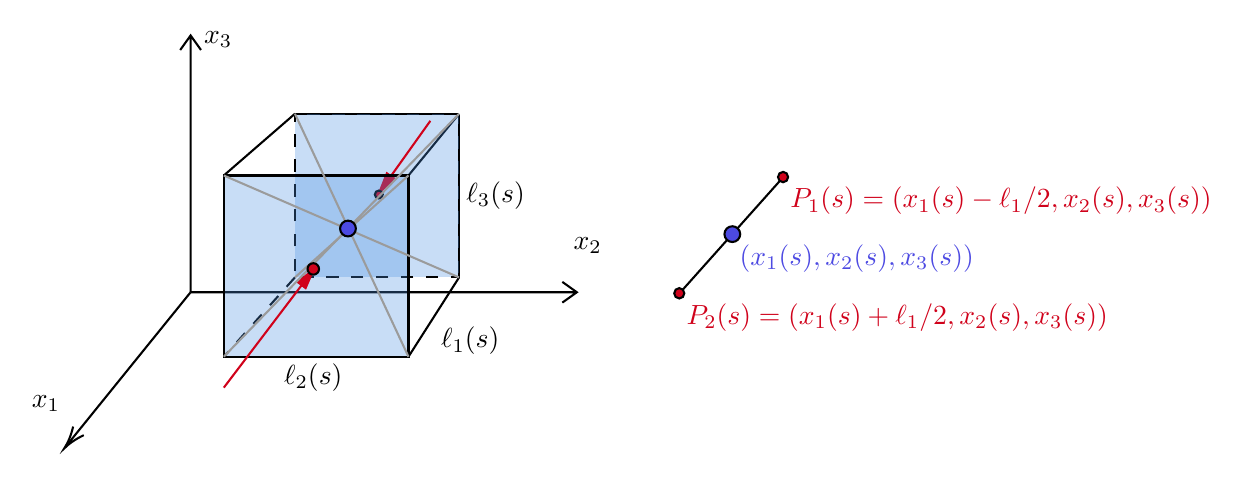
\begin{tikzpicture}[x=0.75pt,y=0.75pt,yscale=-1,xscale=1]
%uncomment if require: \path (0,260); %set diagram left start at 0, and has height of 260

%Shape: Axis 2D [id:dp5041665349843156] 
\draw  (134,170.37) -- (320.09,170.37)(134,46.65) -- (134,170.37) -- cycle (313.09,165.37) -- (320.09,170.37) -- (313.09,175.37) (129,53.65) -- (134,46.65) -- (139,53.65)  ;
%Straight Lines [id:da4518299385759408] 
\draw    (134,170.37) -- (74.35,244.09) ;
\draw [shift={(73.09,245.65)}, rotate = 308.98] [color={rgb, 255:red, 0; green, 0; blue, 0 }  ][line width=0.75]    (10.93,-3.29) .. controls (6.95,-1.4) and (3.31,-0.3) .. (0,0) .. controls (3.31,0.3) and (6.95,1.4) .. (10.93,3.29)   ;
%Straight Lines [id:da9857314894374125] 
\draw    (238.97,201.42) -- (263.35,163.23) ;
%Straight Lines [id:da5801589616872715] 
\draw    (263.35,163.23) -- (263.35,84.37) ;
%Straight Lines [id:da7119304978342444] 
\draw    (238.97,114.11) -- (263.35,84.37) ;
%Straight Lines [id:da8265207937557983] 
\draw    (150,114.11) -- (184.27,84.37) ;
%Straight Lines [id:da5892883478889344] 
\draw    (184.27,84.37) -- (263.35,84.37) ;
%Shape: Rectangle [id:dp31184399621341585] 
\draw  [fill={rgb, 255:red, 74; green, 144; blue, 226 }  ,fill opacity=0.3 ][dash pattern={on 4.5pt off 4.5pt}] (184.27,84.37) -- (263.35,84.37) -- (263.35,163.23) -- (184.27,163.23) -- cycle ;
%Straight Lines [id:da27092452176606474] 
\draw  [dash pattern={on 4.5pt off 4.5pt}]  (184.27,163.23) -- (150,201.42) ;
%Straight Lines [id:da871462086954891] 
\draw [color={rgb, 255:red, 208; green, 2; blue, 27 }  ,draw opacity=1 ]   (249.52,87.77) -- (224.97,122.17) ;
\draw [shift={(223.81,123.8)}, rotate = 305.52] [fill={rgb, 255:red, 208; green, 2; blue, 27 }  ,fill opacity=1 ][line width=0.08]  [draw opacity=0] (12,-3) -- (0,0) -- (12,3) -- cycle    ;
%Shape: Ellipse [id:dp1242803957210763] 
\draw  [fill={rgb, 255:red, 208; green, 2; blue, 27 }  ,fill opacity=1 ] (222.77,123.28) .. controls (222.77,122.23) and (223.62,121.38) .. (224.67,121.38) .. controls (225.72,121.38) and (226.57,122.23) .. (226.57,123.28) .. controls (226.57,124.33) and (225.72,125.18) .. (224.67,125.18) .. controls (223.62,125.18) and (222.77,124.33) .. (222.77,123.28) -- cycle ;
%Shape: Rectangle [id:dp03155729587291001] 
\draw  [color={rgb, 255:red, 0; green, 0; blue, 0 }  ,draw opacity=1 ][fill={rgb, 255:red, 74; green, 144; blue, 226 }  ,fill opacity=0.3 ] (150,114.11) -- (238.97,114.11) -- (238.97,201.42) -- (150,201.42) -- cycle ;
%Straight Lines [id:da13023212112985805] 
\draw [color={rgb, 255:red, 208; green, 2; blue, 27 }  ,draw opacity=1 ]   (150,216.33) -- (193.28,159.36) ;
\draw [shift={(194.49,157.77)}, rotate = 127.22] [fill={rgb, 255:red, 208; green, 2; blue, 27 }  ,fill opacity=1 ][line width=0.08]  [draw opacity=0] (12,-3) -- (0,0) -- (12,3) -- cycle    ;
%Straight Lines [id:da6526415151495846] 
\draw [color={rgb, 255:red, 155; green, 155; blue, 155 }  ,draw opacity=1 ]   (184.27,84.37) -- (238.97,201.42) ;
%Straight Lines [id:da5897939663267662] 
\draw [color={rgb, 255:red, 155; green, 155; blue, 155 }  ,draw opacity=1 ]   (150,114.11) -- (263.35,163.23) ;
%Straight Lines [id:da34056119935146567] 
\draw [color={rgb, 255:red, 155; green, 155; blue, 155 }  ,draw opacity=1 ]   (184.27,163.23) -- (238.97,114.11) ;
%Straight Lines [id:da11549506907395313] 
\draw [color={rgb, 255:red, 155; green, 155; blue, 155 }  ,draw opacity=1 ]   (150,201.42) -- (263.35,84.37) ;

%Shape: Ellipse [id:dp712756393842993] 
\draw  [fill={rgb, 255:red, 76; green, 74; blue, 226 }  ,fill opacity=1 ] (206.02,139.67) .. controls (206.02,137.57) and (207.72,135.87) .. (209.82,135.87) .. controls (211.92,135.87) and (213.62,137.57) .. (213.62,139.67) .. controls (213.62,141.77) and (211.92,143.47) .. (209.82,143.47) .. controls (207.72,143.47) and (206.02,141.77) .. (206.02,139.67) -- cycle ;
%Shape: Ellipse [id:dp8801532139619541] 
\draw  [fill={rgb, 255:red, 208; green, 2; blue, 27 }  ,fill opacity=1 ] (190.34,159.15) .. controls (190.34,157.62) and (191.58,156.38) .. (193.1,156.38) .. controls (194.63,156.38) and (195.87,157.62) .. (195.87,159.15) .. controls (195.87,160.67) and (194.63,161.91) .. (193.1,161.91) .. controls (191.58,161.91) and (190.34,160.67) .. (190.34,159.15) -- cycle ;
%Straight Lines [id:da17829769594080025] 
\draw    (370,170.37) -- (420,114.37) ;
%Shape: Ellipse [id:dp7675769368849501] 
\draw  [fill={rgb, 255:red, 76; green, 74; blue, 226 }  ,fill opacity=1 ] (391.2,142.37) .. controls (391.2,140.27) and (392.9,138.57) .. (395,138.57) .. controls (397.1,138.57) and (398.8,140.27) .. (398.8,142.37) .. controls (398.8,144.47) and (397.1,146.17) .. (395,146.17) .. controls (392.9,146.17) and (391.2,144.47) .. (391.2,142.37) -- cycle ;
%Shape: Ellipse [id:dp2317173269305044] 
\draw  [fill={rgb, 255:red, 208; green, 2; blue, 27 }  ,fill opacity=1 ] (367,170.87) .. controls (367,169.49) and (368.09,168.37) .. (369.44,168.37) .. controls (370.79,168.37) and (371.88,169.49) .. (371.88,170.87) .. controls (371.88,172.25) and (370.79,173.37) .. (369.44,173.37) .. controls (368.09,173.37) and (367,172.25) .. (367,170.87) -- cycle ;
%Shape: Ellipse [id:dp638683839087268] 
\draw  [fill={rgb, 255:red, 208; green, 2; blue, 27 }  ,fill opacity=1 ] (417,114.87) .. controls (417,113.49) and (418.09,112.37) .. (419.44,112.37) .. controls (420.79,112.37) and (421.88,113.49) .. (421.88,114.87) .. controls (421.88,116.25) and (420.79,117.37) .. (419.44,117.37) .. controls (418.09,117.37) and (417,116.25) .. (417,114.87) -- cycle ;

% Text Node
\draw (56,218.77) node [anchor=north west][inner sep=0.75pt]    {$x_{1}$};
% Text Node
\draw (317,142.4) node [anchor=north west][inner sep=0.75pt]    {$x_{2}$};
% Text Node
\draw (139,43.4) node [anchor=north west][inner sep=0.75pt]    {$x_{3}$};
% Text Node
\draw (193.1,203.2) node [anchor=north] [inner sep=0.75pt]    {$\ell _{2}( s)$};
% Text Node
\draw (253.16,185.73) node [anchor=north west][inner sep=0.75pt]    {$\ell _{1}( s)$};
% Text Node
\draw (265.35,123.8) node [anchor=west] [inner sep=0.75pt]    {$\ell _{3}( s)$};
% Text Node
\draw (397,145.77) node [anchor=north west][inner sep=0.75pt]  [color={rgb, 255:red, 77; green, 74; blue, 226 }  ,opacity=1 ]  {$( x_{1}( s) ,x_{2}( s) ,x_{3}( s))$};
% Text Node
\draw (371.44,174.27) node [anchor=north west][inner sep=0.75pt]  [color={rgb, 255:red, 208; green, 2; blue, 27 }  ,opacity=1 ]  {$P_{2}( s) =( x_{1}( s) +\ell _{1} /2 ,x_{2}( s) ,x_{3}( s))$};
% Text Node
\draw (421.44,118.27) node [anchor=north west][inner sep=0.75pt]  [color={rgb, 255:red, 208; green, 2; blue, 27 }  ,opacity=1 ]  {$P_{1}( s) =( x_{1}( s) -\ell _{1} /2 ,x_{2}( s) ,x_{3}( s))$};


\end{tikzpicture}
